\documentclass{article}  
% Include all project wide packages here.
\usepackage{fullpage}
\usepackage{polyglossia}
\setmainlanguage{dutch}
\usepackage{csquotes}
\usepackage{graphicx}
\usepackage{epstopdf}
\usepackage{pdfpages}
\usepackage{caption}
\usepackage[list=true]{subcaption}
\usepackage{float}
%\usepackage{mathtools}
\usepackage{standalone}
\usepackage{import}
\usepackage{tocloft}
\usepackage{wrapfig}
\usepackage{authblk}
\usepackage{array}
\usepackage{booktabs}
\usepackage[toc,page,title,titletoc]{appendix}
\usepackage{xunicode}
\usepackage{amsmath}
\usepackage{fontspec}
\usepackage{unicode-math}
\usepackage[
    backend=bibtexu,
	texencoding=utf8,
bibencoding=utf8,
    style=ieee,
    sortlocale=nl_NL,
    language=auto
]{biblatex}
\usepackage{listings}
\newcommand{\includecode}[3][c]{\lstinputlisting[caption=#2, escapechar=, style=#1]{#3}}
\newcommand{\superscript}[1]{\ensuremath{^{\textrm{#1}}}}
\newcommand{\subscript}[1]{\ensuremath{_{\textrm{#1}}}}


\newcommand{\chapternumber}{\thechapter}
\renewcommand{\appendixname}{Bijlage}
\renewcommand{\appendixtocname}{Bijlagen}
\renewcommand{\appendixpagename}{Bijlagen}

\usepackage[hidelinks]{hyperref} %<--------ALTIJD ALS LAATSTE
  
\renewcommand{\familydefault}{\sfdefault}

\setmainfont[Ligatures=TeX]{Myriad Pro}
\setmathfont{Asana Math}
\setmonofont{Lucida Console}

\usepackage{titlesec, blindtext, color}
\definecolor{gray75}{gray}{0.75}
\newcommand{\hsp}{\hspace{20pt}}
\titleformat{\chapter}[hang]{\Huge\bfseries}{\chapternumber\hsp\textcolor{gray75}{|}\hsp}{0pt}{\Huge\bfseries}
\renewcommand{\familydefault}{\sfdefault}
\renewcommand{\arraystretch}{1.2}
\setlength\parindent{0pt}

%For code listings
\definecolor{black}{rgb}{0,0,0}
\definecolor{browntags}{rgb}{0.65,0.1,0.1}
\definecolor{bluestrings}{rgb}{0,0,1}
\definecolor{graycomments}{rgb}{0.4,0.4,0.4}
\definecolor{redkeywords}{rgb}{1,0,0}
\definecolor{bluekeywords}{rgb}{0.13,0.13,0.8}
\definecolor{greencomments}{rgb}{0,0.5,0}
\definecolor{redstrings}{rgb}{0.9,0,0}
\definecolor{purpleidentifiers}{rgb}{0.01,0,0.01}


\lstdefinestyle{csharp}{
language=[Sharp]C,
showspaces=false,
showtabs=false,
breaklines=true,
showstringspaces=false,
breakatwhitespace=true,
escapeinside={(*@}{@*)},
columns=fullflexible,
commentstyle=\color{greencomments},
keywordstyle=\color{bluekeywords}\bfseries,
stringstyle=\color{redstrings},
identifierstyle=\color{purpleidentifiers},
basicstyle=\ttfamily\small}

\lstdefinestyle{c}{
language=C,
showspaces=false,
showtabs=false,
breaklines=true,
showstringspaces=false,
breakatwhitespace=true,
escapeinside={(*@}{@*)},
columns=fullflexible,
commentstyle=\color{greencomments},
keywordstyle=\color{bluekeywords}\bfseries,
stringstyle=\color{bluestrings},
identifierstyle=\color{purpleidentifiers}
}

\lstdefinestyle{vhdl}{
language=VHDL,
showspaces=false,
showtabs=false,
breaklines=true,
showstringspaces=false,
breakatwhitespace=true,
escapeinside={(*@}{@*)},
columns=fullflexible,
commentstyle=\color{greencomments},
keywordstyle=\color{bluekeywords}\bfseries,
stringstyle=\color{redstrings},
identifierstyle=\color{purpleidentifiers}
}

\lstdefinestyle{xaml}{
language=XML,
showspaces=false,
showtabs=false,
breaklines=true,
showstringspaces=false,
breakatwhitespace=true,
escapeinside={(*@}{@*)},
columns=fullflexible,
commentstyle=\color{greencomments},
keywordstyle=\color{redkeywords},
stringstyle=\color{bluestrings},
tagstyle=\color{browntags},
morestring=[b]",
  morecomment=[s]{<?}{?>},
  morekeywords={xmlns,version,typex:AsyncRecords,x:Arguments,x:Boolean,x:Byte,x:Char,x:Class,x:ClassAttributes,x:ClassModifier,x:Code,x:ConnectionId,x:Decimal,x:Double,x:FactoryMethod,x:FieldModifier,x:Int16,x:Int32,x:Int64,x:Key,x:Members,x:Name,x:Object,x:Property,x:Shared,x:Single,x:String,x:Subclass,x:SynchronousMode,x:TimeSpan,x:TypeArguments,x:Uid,x:Uri,x:XData,Grid.Column,Grid.ColumnSpan,Click,ClipToBounds,Content,DropDownOpened,FontSize,Foreground,Header,Height,HorizontalAlignment,HorizontalContentAlignment,IsCancel,IsDefault,IsEnabled,IsSelected,Margin,MinHeight,MinWidth,Padding,SnapsToDevicePixels,Target,TextWrapping,Title,VerticalAlignment,VerticalContentAlignment,Width,WindowStartupLocation,Binding,Mode,OneWay,xmlns:x}
}

%defaults
\lstset{
basicstyle=\ttfamily\small,
extendedchars=false,
numbers=left,
numberstyle=\ttfamily\tiny,
stepnumber=1,
tabsize=4,
numbersep=5pt
} 
\addbibresource{../../library/bibliography.bib}

\author{Robin Hes (4236815) \and Jorden Kerkhof (3458923)}

\title{EPO3-1 - Opdracht 4: Unified Model Parameters}
\date{3 oktober 2013}
\begin{document}
\maketitle

\section{Abstract}
\label{sec:ump-abstr}

\tableofcontents

\section{Inleiding}
\label{sec:ump-inl}

\section{Probleemstelling}
\label{sec:ump-prob}

\section{Theorie}
\label{sec:ump-theorie}
In SPICE-simulaties wordt uiteraard een model gebruikt, dat een werkelijke transistor zo goed mogelijk nabootst. Een computer rekent immers veel sneller dan een mens en dus is de complexiteit van het model een minder groot probleem. Voor handmatige analyse van een CMOS-transistor is het echter wenselijk om een model te hebben dat ook voor de mens te gebruiken is.
Het unified transistormodel van Rabaey biedt hier een uitkomst. Het model beschrijft, met slechts een enkele vergelijking, de drainstroom $I_{D}$ door de transistor, aan de hand van een vrij beperkt aantal parameters. De drainstroom wordt gemodelleerd in de drie verschillende werkgebieden waarin de transistor zich kan bevinden, wanneer deze in geleiding is, afhankelijk van de spanning over drain en source ($V_{DS}$). Daarnaast beschrijft het model de effecten van velocity saturation.
De vergelijking voor $I_{D}$, zoals gegeven door Rabaey, is als volgt:

\begin{equation}
	I_{D} = k' \frac{W}{L} (V_{GT}V_{min} - \frac{V_{min}^2}{2})(1 + \lambda V_{DS})
	\label{ump-cmos-model-rab}
\end{equation}

Waarbij geldt dat: \\
$$V_{min} = min(V_{GT}, V_{DS}, V_{DSAT})$$
$$V_{GT} = V_{GS} - V_{T}$$
$$V_{T} = V_{T0} + \gamma ( \sqrt{\abs{-2\phi_{F} + V_{SB}}} - \sqrt{\abs{-2\phi_{F}}} )$$
\cite[101]{rabaey-integrated-circuits}\\

Hierin hangen $V_{GS}$, $V_{DS}$ en $V_{SB}$ af van de situatie en zijn $W$, $L$, $k'$, $V_{T0}$, $V_{DSAT}$, $\gamma$, $\lambda$ en $\phi_{F}$ eigenschappen van de transistor.
\\

In sectie \ref{sec:ump-methode} zal de gebruikte methode uiteen gezet worden, om relevante parameters ($k'$, $V_{T0}$, $V_{DSAT}$ en $\lambda$) uit het gegeven model te bepalen, aan de hand van een SPICE-simulatie. Met deze parameters kan vervolgens gerekend worden aan de MOS-transistors uit de bij EPO-3 gebruikte Sea-of-Gates-chip.

\section{Methode}
\label{sec:ump-methode}

Om de voor deze opdracht vereiste parameters te bepalen is er als eerste data nodig om deze uit te bepalen. Dit kunnen metingen aan een daadwerkelijke transistor zijn, maar voor het doel van deze opdracht volstaat het om gegevens uit een SPICE-simulatie te gebruiken. Daarom simuleren we het onderstaande circuit (figuur \ref{fig:ump-sim-circuit}).

\begin{figure}[h]
	\centering
	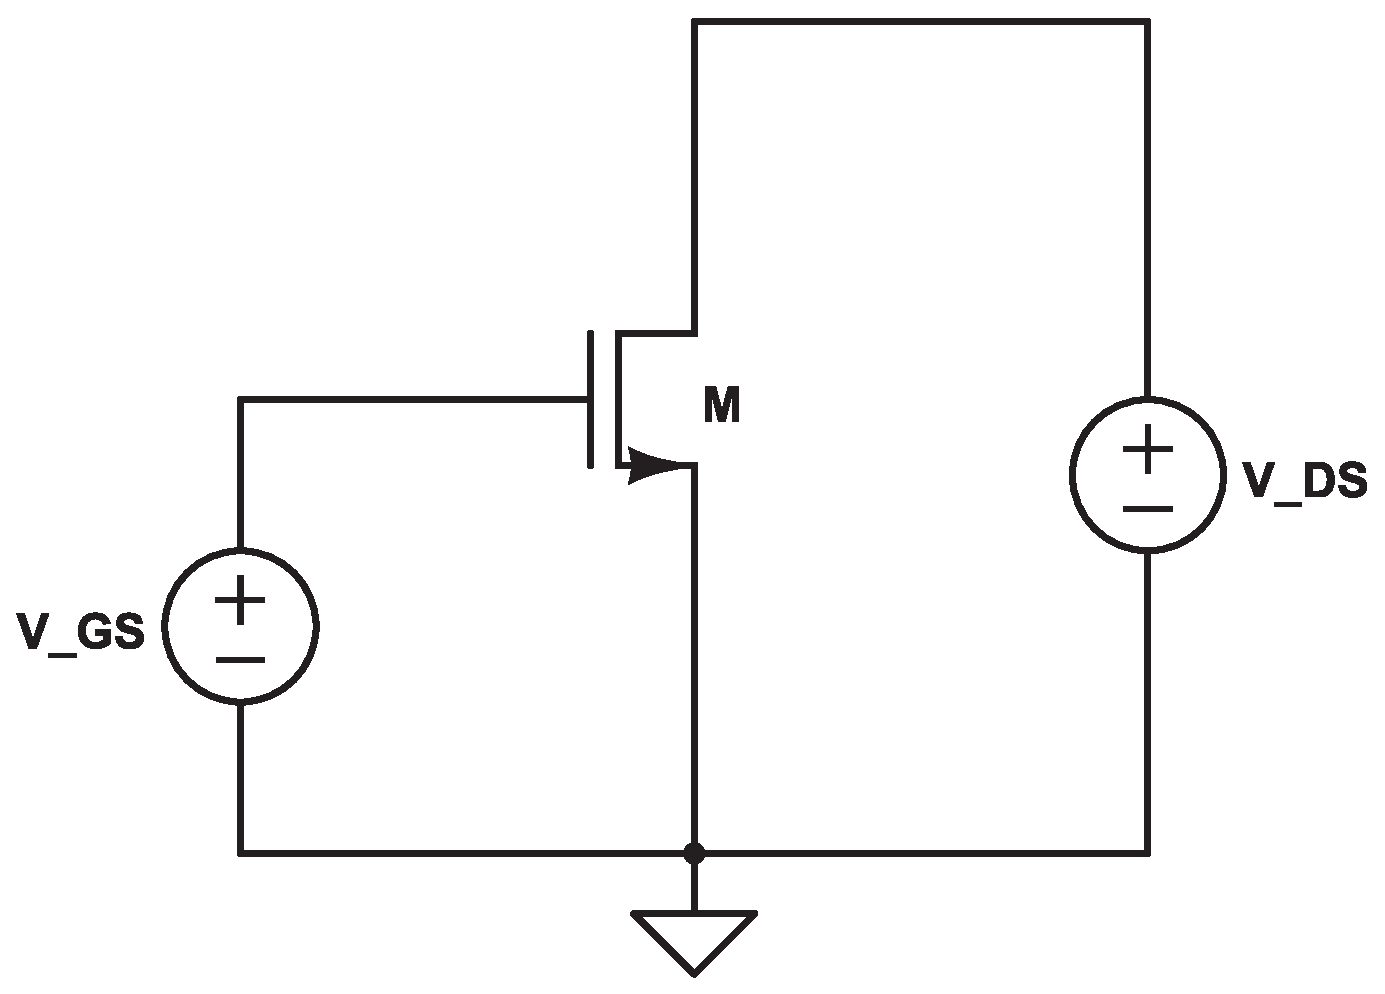
\includegraphics[width=0.5\textwidth]{resource/sim-circuit}
	\caption{Het circuit zoals gebruikt bij simulatie met SPICE}
	\label{fig:ump-sim-circuit}
\end{figure}

Aan de hand van dit circuit kan vervolgens gesimuleerd worden met SPICE. Voor relevante simulatieresultaten kan als eerste een DC-sweep voor $I_{D}$ met als sweepvariabele $V_{DS}$ en tweede parameter $V_{GS}$ worden uitgevoerd en vervolgens een DC-sweep voor $I_{D}$ met als sweepvariabele $V_{GS}$ en als tweede parameter $V_{DS}$.

In dit circuit geldt als randvoorwaarde dat $V_{SB} = 0$, waaruit volgt dat $V_{T} = V_{T0}$ (zie sectie \ref{sec:ump-theorie}).

Gegeven is de volgende vergelijking voor de drainstroom $I_{D}$ door een CMOS-transistor:

\begin{equation}
	I_{D} = \frac{1}{2} k (V_{GS} - V_{T})^2(1 + \lambda V_{DS})
\end{equation}

met

\begin{equation}
	k = k' \frac{W}{L}
\end{equation}

\section{Resultaten}
\label{sec:ump-res}

\section{Conclusie}
\label{sec:ump-conclusie}

\printbibliography

\section{Bijlagen}
\label{sec:ump-bijlagen}


\end{document}
